\documentclass[twoside,b5paper,10pt]{article}
\usepackage{AUTstyle}

\input{kaadam_todo}
\input{Figure/tikz/tikzinit}

\title{PMSM Motor Model for P-HIL Application}
\author{Dávid Kiss}

\institution{Department of Automation and Applied Informatics \\
Budapest University of Technology and Economics}

\email{david.kiss@aut.bme.hu}

\headerTitle{PMSM Motor Model for P-HIL Application \dots}
\headerAuthor{Dávid Kiss}


\begin{document}
\makeAutStyleTitle

\begin{abstract}
Electrical drive simulation is one of the key areas of the emerging trends in power electronics. There are many off-the-shelf solutions available on the market, even engineering tools, like MATLAB/Simulink developed it's own solution for the problem in the Simscape Electrical toolbox. These Solutions however are not open for modification, limiting the field in which they can be used. For motor simulation purposes, different approach seem to be necessary. Real-time execution also crucial in case of HIL\footnote{Hardware-in-the-Loop} and P-HIL\footnote{Power Hardware-in-the-Loop} application.
There are claims, the solutions from different suppliers are applicable for on-line simulation, aiming for HIL and P-HIL environments. This Paper introduces a custom developed motor model, usable for motor emulation and compares it with the PMSM model provided by MATLAB/Simulink.
\end{abstract}


\begin{keywords}
Simulation; PMSM; MATLAB; Real-Time AACS Workshop; 
\end{keywords}

\listoftodos

\section{Introduction}
\label{sec:Introdu}

Electrical drive development is one of the most significant area of the industry nowadays. Intelligent drive modules are penetrating the automotive industry day-by-day. In the traction systems scaling from small power, mild-hybrid applications, to multiple hundred $kW$ Battery Electric Vehicle\footnote{BEV} applications. Electrification is not only present in the drivetrains of the vehicles, but auxiliary devices are started to be electrified as well instead of the pneumatic or hydraulic energy source. Due to the limitations of nowadays battery technology efficiency of all these systems becomes essential factor, due to the direct effects on the vehicle's range.  The emerging number of wind-turbines and renewable energy sources, requires developments in the $MW$ range as well. The rapid development characterizes not just the electrical machines, but the controlling inverters and power conversion devices as well, demanding advancement from the semiconductors and the embedded computation units as well. With today's \emph{SiC} and \emph{GaN} semiconductors, switching frequencies in the $100\ kHz$ range becoming usual.

The market and the competition demands fast, reliable and inexpensive development of new technologies. Development processes without simulation tools are not sustainable. Complex systems, like a vehicles drivetrain comes together with the interaction of multiple parts, like the battery or other power sources, the power converter and the control software inside it, the electrical machine, and the mechanical drivetrain behind that. These components cannot be handled independently, one design decision in on component can affect several others, the development of them has to be run simultaneously, as an iterative process. During the design off-line simulation tools are used in wide range. Mathematical modeling for control softwares and for electrical design. and FEM\footnote{Finite Element Model} for magnetic and mechanical design. In later stages, on-line simulation tools becomes important to validate and test each component and software before system integration.

HIL Simulators are widely used in control software development, especially in Power Electronics. The reliability and stability of the control structures and protection features are essential to be checked in a non-destructive environment. Testing on real hardware is usually expensive, can be destructive in case of unintended short-circuits and over currents. These faults in high power ranges can result in substantial material loss or even endangering human life. Signal level HIL simulators are simulating the environment for the control hardware, usually based on FPGA(s), providing a real-time test environment. These simulation environments are taking the controls signals from the ECU as their inputs and producing the proper feedback signals, whether they are digital or analogue. These environments can be completely transparent for the DUT\footnotes{Device Under Test}, and validations methods are available for them\change{Tamás cikkét be kell hivatkozni}.

The author aiming to extend this approach to provide test environment for the Power Electronics as well, excluding only the mechanical and moving parts from the system. The added value lies within the opportunity to include the parasitic effects in the hardware design and the real control latencies of the sensors, testing also the thermal stability of the system. Emulating the rotating machine with an electrical unit removes the complexity and cost of coupling two electrical machines together, which are especially dangerous with high rotation speeds and large masses. The power efficiency is also good, the electrical power can be circulated within the system, only the losses have to fed in for external source. Efficiency and loss analysis can be conducted more detailed with the P-HIL approach as well. To be able to simulate the electrical machine for the DUT, conventional motor models with Voltage input, current and torque output are not comprehensive enough, more internal variables have to be available, like generated phase voltages. In this paper, a model meeting this goal is presented and validated with the motor model included in Matlab/Simulink.

The following chapters of this paper are organized as follows: \sectionname~\ref{sec:matPMSM} briefly introduce the modeling technique behind the PMSM machine and discusses the parameters of the example machine. \sectionname~\ref{sec:simulink_model} investigates the PMSM motor model available in MATLAB/Simulink (r2019b) SimScape Electrical toolbox. \sectionname~\ref{sec:custom_model} introduces the model solution implemented by the author. In \sectionname~\ref{sec:test_framework} the test environment and the test cases are introduced. The simulation results are summarized and evaluated in \sectionname~\ref{sec:results}. Finally, in \sectionname~\ref{sec:conclusion} the following steps will be introduced with a brief outlook to the author goals. 

\todo[inline]{Át kell még nézni.}

\section{Mathematical model of a PMSM Machine}
\label{sec:matPMSM}

The Automotive industry always played a key role in innovation and always pioneered with new and emerging technologies. The situation is no different in the case of electrification nowadays. Electrical motors are the core element of modern hybrid (HEV) and Battery Electric Vehicle's (BEV) drivetrains. Volume and mass is a very limiting factor, especially in the case of BEV vehicles, because the saved mass and volume provides more space for the battery itself, providing higher range for the vehicle. Because of these reasons, 3-phase induction (IM\footnote{Induction Machine}) and PMSM\footnote{Permanent Magnet Synchronous Machine} machines are commonly used in traction (and other actuation) systems in the automotive industry. The difference between these two type of electrical machines is the source of the magnetic flux inside. In the case of the IM the magnetic field has to come from external excitation, in the PMSM machine, as the name suggests, the magnetic field is generated by the built-in permanent magnets. PMSM machines are especially superior in power density, however their drawback is the necessity of complex control algorithms and the expensive magnetic material.

There are multiple construction variables within the group of PMSM motors, these distinctions can affect the mathematical models as well. Regarding to the rotor configuration, one can differentiate between the \emph{non-salient pole} machines, and the \emph{salient pole} machines, showed on Figure \ref{fig:mot_sailient_non}

The non-salient pole machines are usually equipped with surface mount magnets on their rotors. The simplicity of the manufacturing made the configuration popular. The air gap between the rotor and the stator is homogeneous, which means the inductance is not dependent on the rotor position, so  $L_d$ and the $Lq$ are equal. The magnets are more exposed to demagnetisation and in case of high speed rotors, the magnets can become loose due to the centripetal forces.

 \begin{figure}[h]
        \centering
%%----start of first subfigure----
        \subfloat[Interior magnets]{
            \label{subfig:one} %% label for first subfigure
            \includegraphics[width=0.2\linewidth]{Figure/motor_interior.pdf}}
        \hspace{0.02\linewidth}
%%----start of second subfigure----
        \subfloat[Surface mounted magnets]{
            \label{subfig:two} %% label for second subfigure
            \includegraphics[width=0.2\linewidth]{Figure/motor_exterior.pdf}}
        \caption{PMSM Motor types}
        \label{fig:mot_sailient_non} %% label for entire figure
\end{figure}

The \emph{salient pole} machines have their magnets embedded inside the material of the rotor, leading to a magnetic field which is not uniform in the air gap, meaning the inductance is depending from the rotor position, so $L_d\ \ne{}\ L_q$. The configuration have more complexity in production, however the rotor has superior mechanical integrity over the surface mount magnet type. The ratio of the $L_d$ and $L_q$ inductances can be set by the angles of the magnets. Sensorless motor control algorithms are simpler and more robust with salient pole machines.

Other differentiate is the shape of the Back-EMF voltage, which is dependent on the spatial configuration of the stator windings. There are machines with sinusoidal electromotive force profile, and there are machines with trapezoidal EMF profile. \unsure{Itt talán még van tér a fejlődésre, vagy ki kell hagyni teljesen.}

\info[inline]{Itt még be kell hivatkozni Veszprémi könyvét meg írni arról, hogy miért király a PMSM!}


This paper details the mathematical description of the PMSM due to it's simplicity, with the following assumptions:
\begin{itemize}
  \item The machine is symmetrical, non-salient pole. ($L_d = L_q$)
  \item The stator winding are in star connection
  \item Losses are neglected (Ventilation, internal friction, iron losses)
  \item Coil inductance and resistances are constant
\end{itemize}

To derive the equations describing a PMSM machine, it worth to take a look on the external excitation DC machine, presented on Fig. \ref{fig:dc_machine}.

\begin{figure}[htb]
\begingroup
\tikzset{}
 \centerline{\includegraphics[width=.35\columnwidth]{.//Figure/dc_mot_veszpr.png}}
 \endgroup
 \caption{External excitation DC machine}
 \label{fig:dc_machine}
\end{figure}

From the equivalent circuit, Eq. \ref{eq:dc_dt} can be deducted. These Equations describing the relationship between the motor input voltage, current, torque and speed.

\begin{gather}
\begin{align*} 
\label{eq:dc_dt}
u(t) &= Ti(t) + L\frac{di(t)}{dt} + u_b(t) \\ 
u_b(t) &= k\Phi{}\omega{}(t) \\
m(t) - m_t(t) &= \Theta{}\frac{d\omega{}(t)}{dt} \\
m(t) &= k\Phi{}i(t) \\
\omega{}(t) &= \frac{d\alpha(t)}{dt}
\end{align*}
\end{gather}

The electrical difference between the stator of a PMSM and a DC motor, the PMSM has a 3-phase winding with the spatial displacement of $\deg{120}$, connected in star. Each phase can modelled as a series RL and a voltage source. 

\begin{figure}[htb]
\begingroup
\tikzset{}
 \centerline{\includegraphics[width=.35\columnwidth]{.//Figure/threephase_winding.pdf}}
 \endgroup
 \caption{The equvalent circuit of a 3-phase motor winding}
 \label{fig:threephase_winding}
\end{figure}

If there no alternative current conducting path, other than the three phase connection (No parasitic coupling or short to earth), the 3-phase current system is symmetrical, meaning $I_A + I_B + I_C = 0$, thus the current phasor can be described with two independent values instead of three. To utilize this simplification, the Clark transformation is utilised, presented on Eq. \ref{eq:clark}

\begin{gather}
\label{eq:clark}
    \begin{bmatrix}
    \alpha \\ \beta \\ 0
    \end{bmatrix}
    =
    \frac{2}{3}
    \begin{bmatrix}
    1 & -\frac{1}{2} & -\frac{1}{2} \\[0.5em]
    0 & \frac{\sqrt{3}}{2} & -\frac{\sqrt{3}}{2} \\[0.5em]
    \frac{1}{2} & \frac{1}{2} & \frac{1}{2}
    \end{bmatrix}
    \begin{bmatrix}
    a \\ b \\ c
    \end{bmatrix}
\end{gather}

To get back the values in the original 3-phase reference frame, the Inverse-Clark transformation (Eq. \ref{eq:inv_clark}.) is used.

\begin{gather}
\label{eq:inv_clark}
    \begin{bmatrix}
     a \\ b \\ c
    \end{bmatrix}
    =
    \begin{bmatrix}
    1            & 0                  & 1             \\[0.5em]
    -\frac{1}{2} & \frac{\sqrt{3}}{2} & 1             \\[0.5em]
    -\frac{1}{2} & -\frac{\sqrt{3}}{2}& 1
    \end{bmatrix}
    \begin{bmatrix}
     \alpha \\ \beta \\ 0
    \end{bmatrix}
\end{gather}

Parameters and variables van be dependent on the angular position of the rotor, which can lead to numerically complexity. One can transform the equations from the $\alpha\beta$ reference frame, tied to the stator. to a rotating reference frame, tied to the rotor, the so called $dq$ reference frame. By doing this, the motor equations becomes independent from the position of the rotor, enclosing the trigonometric calculations inside the transformation. The transformation from the $\alpha{}\beta{}$ to the $dq$ reference frame is called the Park transformation, described in Eq. \ref{eq:clark}.

\begin{gather}
\label{eq:park}
    \begin{bmatrix}
    d\\ q \\ 0
    \end{bmatrix}
    =
    \frac{2}{3}
    \begin{bmatrix}
    sin(\theta) & sin(\theta-\frac{2\pi}{3}) & sin(\theta+\frac{2\pi}{3}) \\[0.5em]
    cos(\theta) & cos(\theta-\frac{2\pi}{3}) & cos(\theta+\frac{2\pi}{3}) \\[0.5em]
    \frac{1}{2} & \frac{1}{2}                & \frac{1}{2}
    \end{bmatrix}
    \begin{bmatrix}
    a \\ b \\ c
    \end{bmatrix}
\end{gather}

The transformation used to calculate the valued and equations within the $\alpha{}\beta{}$ reference frame from the $dq$ reference frame is the Inverse-Clark transformation, described in Eq. \ref{eq:inv_clark}. 

\begin{gather}
\label{eq:inv_park}
    \begin{bmatrix}
    a \\ b \\ c
    \end{bmatrix}
    =
    \begin{bmatrix}
    sin(\theta)                & cos(\theta)                & 1                   \\[0.5em]
    sin(\theta-\frac{2\pi}{3}) & cos(\theta-\frac{2\pi}{3}) & 1                   \\[0.5em]
    sin(\theta+\frac{2\pi}{3}) & cos(\theta+\frac{2\pi}{3}) & 1
    \end{bmatrix}
    \begin{bmatrix}
    d\\ q \\ 0
    \end{bmatrix}
\end{gather}



The Clark and the Inverse-Clarke transformation can be used equivalently with changing the direction of the rotation angle.

 \begin{figure}[h]
        \centering
%%----start of first subfigure----
        \subfloat[Stator Reference frame]{
            \label{subfig:one} %% label for first subfigure
            \includegraphics[width=0.3\linewidth]{Figure/coord_abc.pdf}}
        \hspace{0.02\linewidth}
%%----start of second subfigure----
        \subfloat[$\alpha\beta$ and $dq$ Reference frame]{
            \label{subfig:two} %% label for second subfigure
            \includegraphics[width=0.3\linewidth]{Figure/coord_alpha_dq.pdf}}
        \caption{Different reference frames}
        \label{fig:bme} %% label for entire figure
\end{figure}


In the $dq$ reference frame the equivalent circuit model of a PMSM machine looks the following:

\todo[inline]{Ábra a PMSM helyettesítő képről}

The equation describing the electrical and mechanical behavior of the motor are presented in...

\todo[inline]{Motor egyenelneltek}

Key parameters of the simulated motor in this paper can be found in \ref{tab:machine}.

\begin{table}[htb]
\caption{Parameters of the example machine}
\begin{center}
\begin{tabular}{|r|c|c|}
\hline
\textbf{Parameter} & \textbf{Symbol} & \textbf{Value} \\
\hline
Nominal Power & $P_N$ & $90\ kW$ \\
\hline
Nominal RMS Voltage & $U_N$ & $400\ V$ \\
\hline
Nominal frequency & $f_N$ & $100\ Hz$ \\
\hline
Winding resistance & $R_s$ & $35.6\ m\Omega$ \\
\hline
Winding Inductance & $L\ =\ L_d\ =\ L_q$& $565.8\  \mu{}H$ \\
\hline
Motor Inertia & $\Theta$ & $0.0912\  kg\cdot{}m^2$ \\
\hline
Motor pole pairs & $pp$ & $1$ \\
\hline
Inverter Switching frequency & $f_{sw}$ & $5\ kHz$ \\
\hline
\end{tabular}
\end{center}
\label{tab:machine}
\end{table}

The parameters were chosen to suit the Invert which will be used during the measurements. This is a 2-level, 3-phase inverter with $140\ kW$ electrical power. Due to the low switching frequency, the external coupling inductance will be selected to meet the motor inductance, and the role of the inverter will be to simulate the motor Back-EMF voltage, in the upcoming work of the author.
\section{The Simulink Built-In Implementation}
\label{sec:simulink_model}

MATLAB/Simulink is one of the most popular computation and numerical modelling tool available on the market. Simulink is a graphical modeling platform in which one can solve differential equation systems within an interactive graphical interface. Simulink has multiple toolboxes and extensions, one of them is the Simscape package, which hides the equations from the model developer, and provide a more abstract environment in specialised areas of engineering like mechanical, thermal, or electrical simulations. Simscape models are compatible with HDL code generation, which makes them compatible with real time, FPGA based simulation. The Simulink icon of the available PMSM motor model is presented on Fig. \ref{fig:pmsm_simulink}..

\begin{figure}[htb]
\begingroup
\tikzset{}
 \centerline{\includegraphics[width=.35\columnwidth]{.//Figure/pmsm_simulink.png}}
 \endgroup
 \caption{Simscape Electrical PMSM model}
 \label{fig:pmsm_simulink}
\end{figure}

On the input side, it has two electrical conserving ports, one marked with $~$, representing the three-phase input connection and one marked with $n$, representing the neutral point connection, which is necessary to close the electrical circuit for the zero order current components. On the output side, it has two mechanical conserving ports, one marked with $R$, representing the rotor of the motor, and on marked with $C$, representing the case of the motor.

The winding configuration of the motor is configurable between star and delta configuration. Avaliable, user configurable electrical parameters parameters are the following:
\begin{itemize}
    \item Number of pole pairs
    \item Permanent magnet flux linkage
    \item Stator $d$-axis inductance
    \item Stator $q$-axis inductance
    \item Zero-sequence inductance
    \item Stator resistance per phase
\end{itemize}

Mechanical parameters can be set for the specific application as well:

\begin{itemize}
    \item Rotor inertia
    \item Rotor damping
\end{itemize}

Unfortunately the implementation of the internal model is hidden from the user, the documentation describes the equations behind the model. The equtions are also in $dq$ reference frame, and presented in Eq. \ref{eq:matlab_motor}

\begin{align*}
\label{eq:matlab_motor_elec}
    v_d &= R_si_d + L_d\frac{di_d}{dt}-N\omega{}i_qL_q \\
    v_q &= R_si_q + L_q\frac{di_q}{dt}+N\omega{}(i_qL_q+\psi_m) \\
    v_0 &= R_si_0 + L_0\frac{di_0}{dt}
\end{align*}

The mechanical torque is calculated as follows:

\begin{equation}
\label{eq:matlab_motor_mech}
    T &= \frac{3}{2}N(i_q(i_dL_d + \psi{}_m) - i_di_qL_q) \\
\end{equation}

It can be seen that the internal EMF voltages are not accessible for the user. This limiation excludes the possibility to use it in the P-HIL enviroment.


\section{The Custom Implementation}
\label{sec:custom_model}

The motor model implemented by the author is also made in MATLAB/Simulink, but not with the Simscape Electrical toolbox, only with ordinary differential equations. The mathematical description meets the presented equations in \sectionname~\ref{sec:matPMSM}.

\section{Test Framework}
\label{sec:test_framework}



\section{Result of Comparison}
\label{sec:results}


\begin{figure}[htb]

\subfloat[Custom implementation]{%
  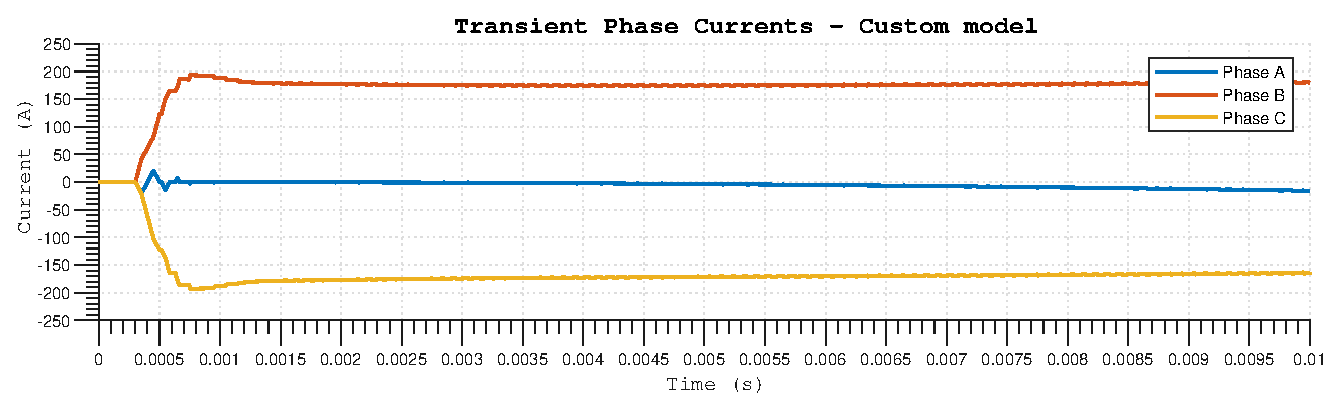
\includegraphics[width=1\columnwidth]{.//Figure/EPS/custom_phase_currents.eps}%
}

\subfloat[Simscape Implementation]{%
  \includegraphics[width=1\columnwidth]{.//Figure/EPS/PE_phase_currents.eps}%
}

\label{fig:Transient_currents}
\caption{Transient Currents}

\end{figure}


\begin{figure}[htb]

\subfloat[Custom implementation]{%
  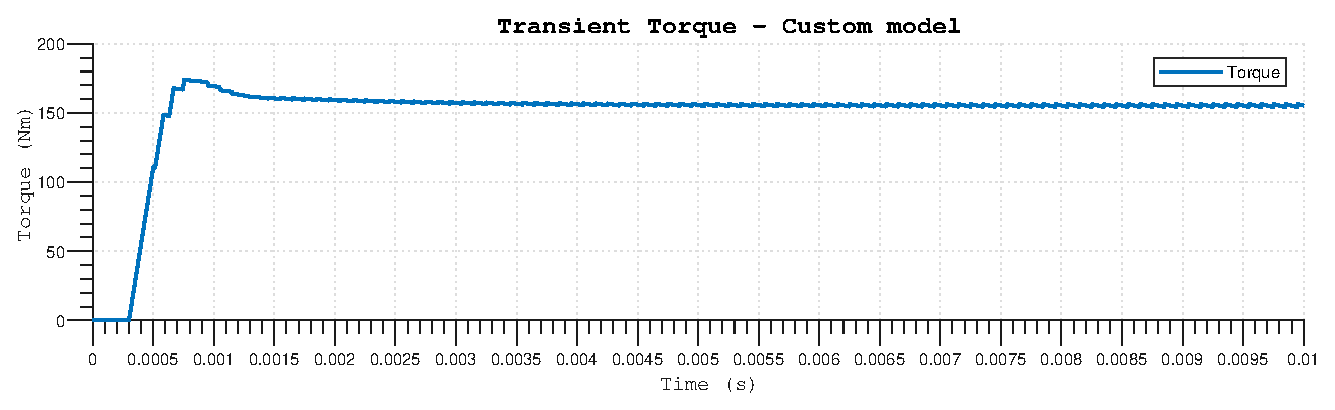
\includegraphics[width=1\columnwidth]{.//Figure/EPS/custom_torque.eps}%
}

\subfloat[Simscape Implementation]{%
  \includegraphics[width=1\columnwidth]{.//Figure/EPS/PE_torque.eps}%
}

\label{fig:Transient_torque}
\caption{Transient Torques}

\end{figure}





\begin{figure}[htb]

\subfloat[Custom currents]{%
  \includegraphics[width=1\columnwidth]{.//Figure/EPS/custom_speedramp_currents.eps}%
}

\subfloat[PE currents]{%
  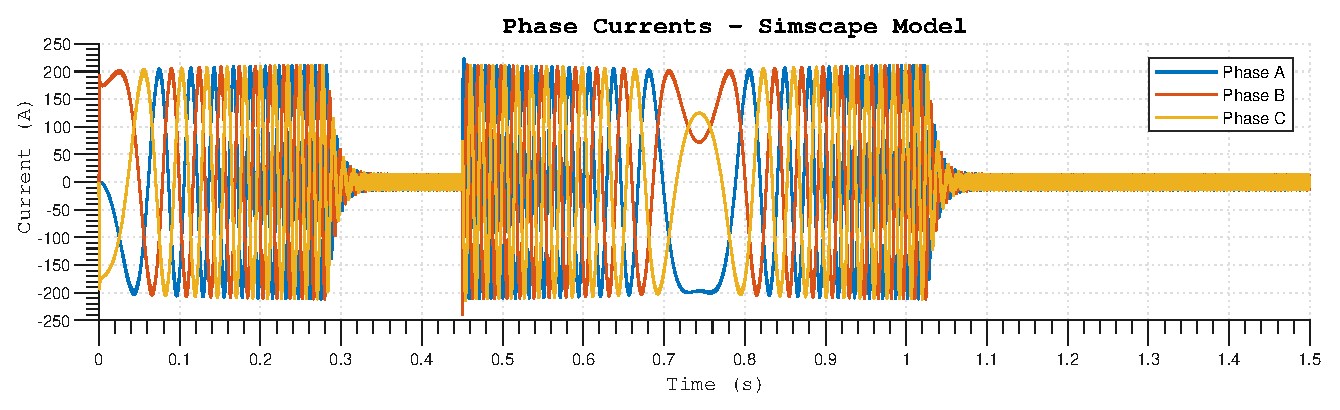
\includegraphics[width=1\columnwidth]{.//Figure/EPS/pe_speedramp_currents.eps}%
}

\subfloat[Error currents]{%
  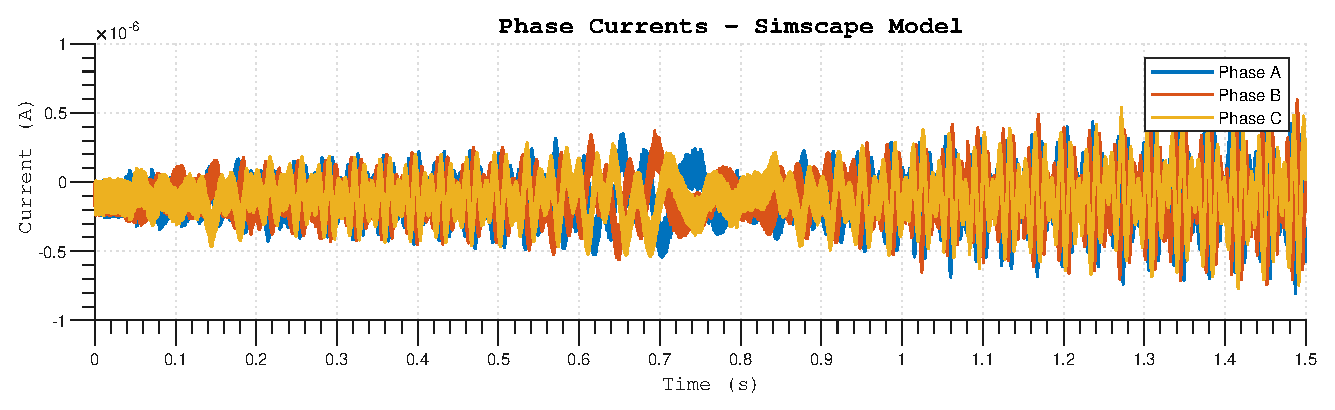
\includegraphics[width=1\columnwidth]{.//Figure/EPS/err_speedramp_currents.eps}%
}


\label{fig:speedramp_currents}
\caption{Phase Currents}

\end{figure}



\section{Conclusion}
\label{sec:conclusion}


\section{Bibliography}
\label{sec:bib}

\section*{Acknowledgments}
 { \small The author would like to express his thanks to Dr. István Varjasi for his support as a scientific advisor.
This work has been supported by the Department of Automation and Applied Informatics}

\makeAutBib{reni,itemsetmining}

\end{document}
